\documentclass[10pt]{beamer}
\usetheme[progressbar=frametitle]{metropolis} 
\setbeamertemplate{frame numbering}[fraction]
\setbeamertemplate{footline}{\insertshorttitle\insertshortsubtitle\hfill\insertshortauthor\hspace*{2em}\insertframenumber/\inserttotalframenumber\hspace*{2em}\vskip2pt}
% Packages
\usepackage{graphicx}
\usepackage{amsmath}
\usepackage{hyperref}
\usepackage{amsthm}
\usepackage{tikz}
\usepackage[spanish]{babel}

\usepackage[most]{tcolorbox}

% Environments and boxes
\newtcolorbox{cajita}[1][]{
	#1
}

\newenvironment{sol}
{\renewcommand\qedsymbol{$\square$}\begin{proof}[\textbf{Solución.}]}
	{\end{proof}}

\newenvironment{dem}
{\renewcommand\qedsymbol{$\blacksquare$}\begin{proof}[\textbf{Demostración.}]}
	{\end{proof}}

\newtheorem{problema}{Problema}
\newtheorem{definicion}{Definición}
\newtheorem{ejemplo}{Ejemplo}
\newtheorem{teorema}{Teorema}
\newtheorem{corolario}{Corolario}[teorema]
\newtheorem{lema}[teorema]{Lema}
\newtheorem{prop}{Proposición}
\newtheorem*{nota}{\textbf{NOTA}}
\renewcommand\qedsymbol{$\blacksquare$}

% Set color of title, subtitle, author, institute, and date to white
\setbeamercolor{title}{fg=white}
\setbeamercolor{subtitle}{fg=white}
\setbeamercolor{author}{fg=white}
\setbeamercolor{institute}{fg=white}
\setbeamercolor{date}{fg=white}
% Title Page

\title{ Geometría diferencial}
\subtitle{ - Superficies mínimas: Scherk 1 y Scherk 2 }
\author{Rudik Rompich}
\institute{Universidad del Valle de Guatemala }
\date{\today}

\begin{document}

\usebackgroundtemplate{

\includegraphics[width=\paperwidth,height=\paperheight]{imagenes/wallpaper.png}
}
\maketitle

\usebackgroundtemplate{}


\begin{frame}{Índice}
\setbeamertemplate{section in toc}[sections numbered]
\tableofcontents[hideallsubsections]
\end{frame}

\section{Introducción }


\section{Historia y parametrizaciones }

  %------------------------
  \begin{frame}{Historia de las superficies de Scherk 1 y Scherk 2}
    
    \begin{itemize}
      \item Las superficies de Scherk llevan el nombre de Heinrich Scherk, nacido el 27 de octubre de 1798 en Posen, Prusia (ahora Poznań, Polonia), y fallecido el 4 de octubre de 1885\footnote{Fuente: \url{https://mathshistory.st-andrews.ac.uk/Biographies/Scherk/}}.
      \item Describió las dos superficies mínimas completas incrustadas, la primera superficie de Scherk y la segunda superficie de Scherk, en 1834\footnote{Fuente: \url{https://en.wikipedia.org/wiki/Scherk_surface}}.
    \end{itemize}
    \end{frame}
    
    \begin{frame}{Historia de las superficies de Scherk 1 y Scherk 2}
    \begin{itemize}
      \item La primera superficie de Scherk es asintótica a dos familias infinitas de planos paralelos, ortogonales entre sí. Estos planos se encuentran cerca de $z = 0$ en un patrón de tablero de ajedrez de arcos de puente\footnote{Fuente: \url{https://en.wikipedia.org/wiki/Scherk_surface}}.
    \end{itemize}
    \end{frame}

    \begin{frame}{Scherk 1}

      \begin{itemize}
        \item Para un número natural $n$, encontar una superficien miníma $\Sigma_n$, definida en
        $$
        u_n:\left(-\frac{\pi}{2},+\frac{\pi}{2}\right) \times\left(-\frac{\pi}{2},+\frac{\pi}{2}\right) \rightarrow \mathbb{R}
        $$
        tal que 
        $$
        \begin{aligned}
        & \lim _{y \rightarrow \pm \pi / 2} u_n(x, y)=+n \text { para }-\frac{\pi}{2}<x<+\frac{\pi}{2} \\
        & \lim _{x \rightarrow \pm \pi / 2} u_n(x, y)=-n \text { paras }-\frac{\pi}{2}<y<+\frac{\pi}{2}
        \end{aligned}
        $$
       
    
      \end{itemize}
      
    \end{frame}

    \begin{frame}{Scherk 1}
      ¿Qué pasa si $n$ tiende a infinito? 
    
    \end{frame}
    \begin{frame}{Scherk 1}
      La respuesta la dio Scherk in 1834: la superficie cuando $n$ tiene al infinito es $\Sigma$ definida como: 
        $$
        \begin{aligned}
        & u:\left(-\frac{\pi}{2},+\frac{\pi}{2}\right) \times\left(-\frac{\pi}{2},+\frac{\pi}{2}\right) \rightarrow \mathbb{R}, \\
        & u(x, y)=\log \left(\frac{\cos (x)}{\cos (y)}\right) .
        \end{aligned}
        $$
        La superficie de Scherk 1 sobre el cuadrado
        $$
        \Sigma=\left\{\left(x, y, \log \left(\frac{\cos (x)}{\cos (y)}\right)\right) \in \mathbb{R}^3 \mid-\frac{\pi}{2}<x, y<+\frac{\pi}{2}\right\}
        $$
    \end{frame}

    \begin{frame}{Scherk 1}
      \begin{figure}[H]
        \centering
        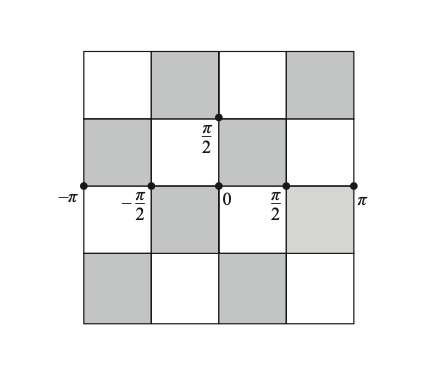
\includegraphics[scale=.4]{imagenes/8}
        \caption{Grid en el que se define}
      \end{figure}
      \end{frame}


    \begin{frame}{Scherk 1}
      \begin{figure}[H]
        \centering
        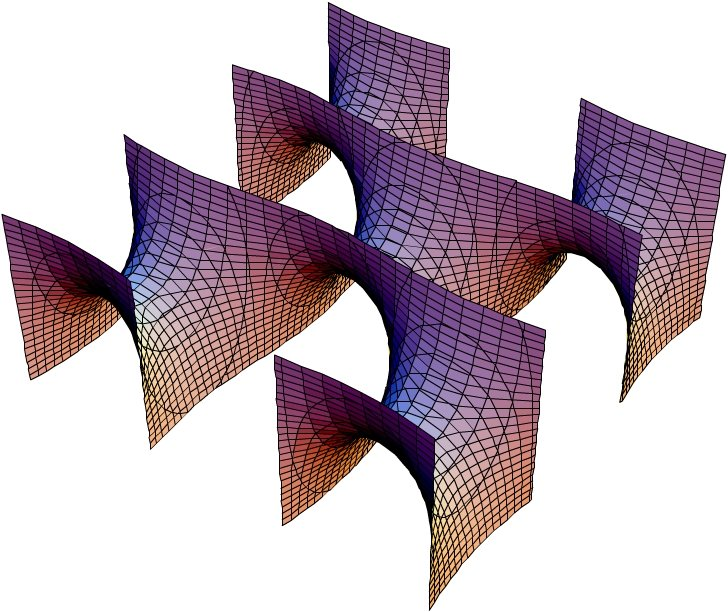
\includegraphics[scale=.4]{imagenes/4}
        \caption{$\mathbf{x}(u,v)=(u,v, \log \left(\frac{\cos u}{\cos v}\right))$}
      \end{figure}
      \end{frame}


      \begin{frame}{Scherk 1 (el de verdad)}
        \begin{align*}
          &\mathbf{x}(u, v)=\left(\arg \frac{\zeta+i}{\zeta-i}, \arg \frac{\zeta+1}{\zeta-1}, \log \left|\frac{\zeta^2+1}{\zeta^2-1}\right|\right),\\
          &\zeta \neq \pm 1, \zeta \neq \pm i
          \end{align*}
        \end{frame}

    \begin{frame}{Historia de las superficies de Scherk 1 y Scherk 2}
      \begin{itemize}
        \item La segunda superficie de Scherk se parece globalmente a dos planos ortogonales cuya intersección consta de una secuencia de túneles en direcciones alternas\footnote{Fuente: \url{https://en.wikipedia.org/wiki/Scherk_surface}}.
        \item Tiene la ecuación implícita $\sin(z) - \sinh(x)\sinh(y)=0$ y puede ser parametrizada como  $x(r,\theta) = 2 \Re ( \ln(1+re^{i \theta}) - \ln(1-re^{i \theta}) ) = \ln \left( \frac{1+r^2+2r \cos \theta}{1+r^2-2r \cos \theta} \right)$, $y(r,\theta) = \Re ( 4i \tan^{-1}(re^{i \theta})) = \frac{1+r^2-2r \sin\theta}{1+r^2+2r \sin \theta} $, $z(r,\theta) = \Re ( 2i(-\ln(1-r^2e^{2i \theta}) + \ln(1+r^2e^{2i \theta}) ) = 2 \tan^{-1}\left( \frac{2 r^2 \sin 2\theta}{r^4} \right)$.
      \end{itemize}
      \end{frame}
      \begin{frame}{Scherk 2}
        \begin{figure}[H]
          \centering
          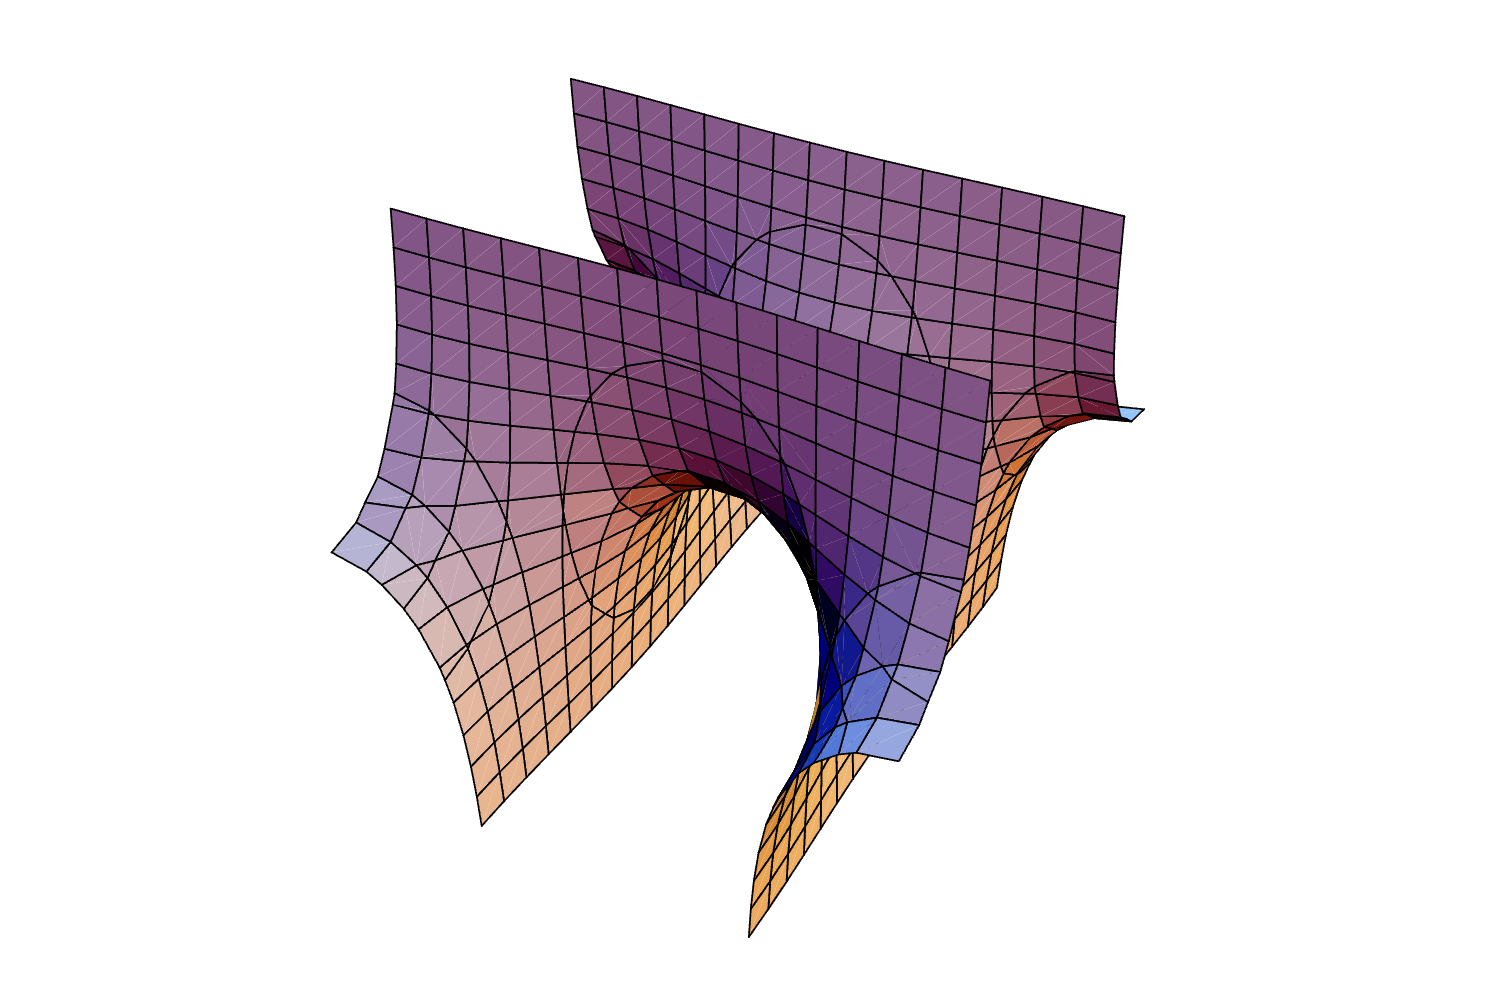
\includegraphics[scale=.3]{imagenes/5.png}
          \caption{$\mathbf{x}(u,v)=( \ln \left( \frac{1+r^2+2r \cos \theta}{1+r^2-2r \cos \theta} \right), \frac{1+r^2-2r \sin\theta}{1+r^2+2r \sin \theta} , 2 \tan^{-1}\left( \frac{2 r^2 \sin 2\theta}{r^4} \right))$}
        \end{figure}
        \end{frame}
      \begin{frame}{Historia de las superficies de Scherk 1 y Scherk 2}
        \begin{itemize}
          \item En 2006, Harold Rosenberg y Pascal Collin utilizaron superficies hiperbólicas de Scherk para construir un difeomorfismo armónico desde el plano complejo al plano hiperbólico, refutando así la conjetura de Schoen-Yau.
        \end{itemize}
        \end{frame}

        \begin{frame}{Historia de las superficies de Scherk 1 y Scherk 2}
          \begin{itemize}
            \item El trabajo de Scherk sobre superficies mínimas no solo es significativo en matemáticas sino también en las artes. El artista estadounidense Brent Collins ha basado muchas de sus esculturas en la segunda superficie mínima de Scherk.
          \end{itemize}
          \end{frame}

          \begin{frame}{Brent Collins}
            \begin{figure}[H]
              \centering
              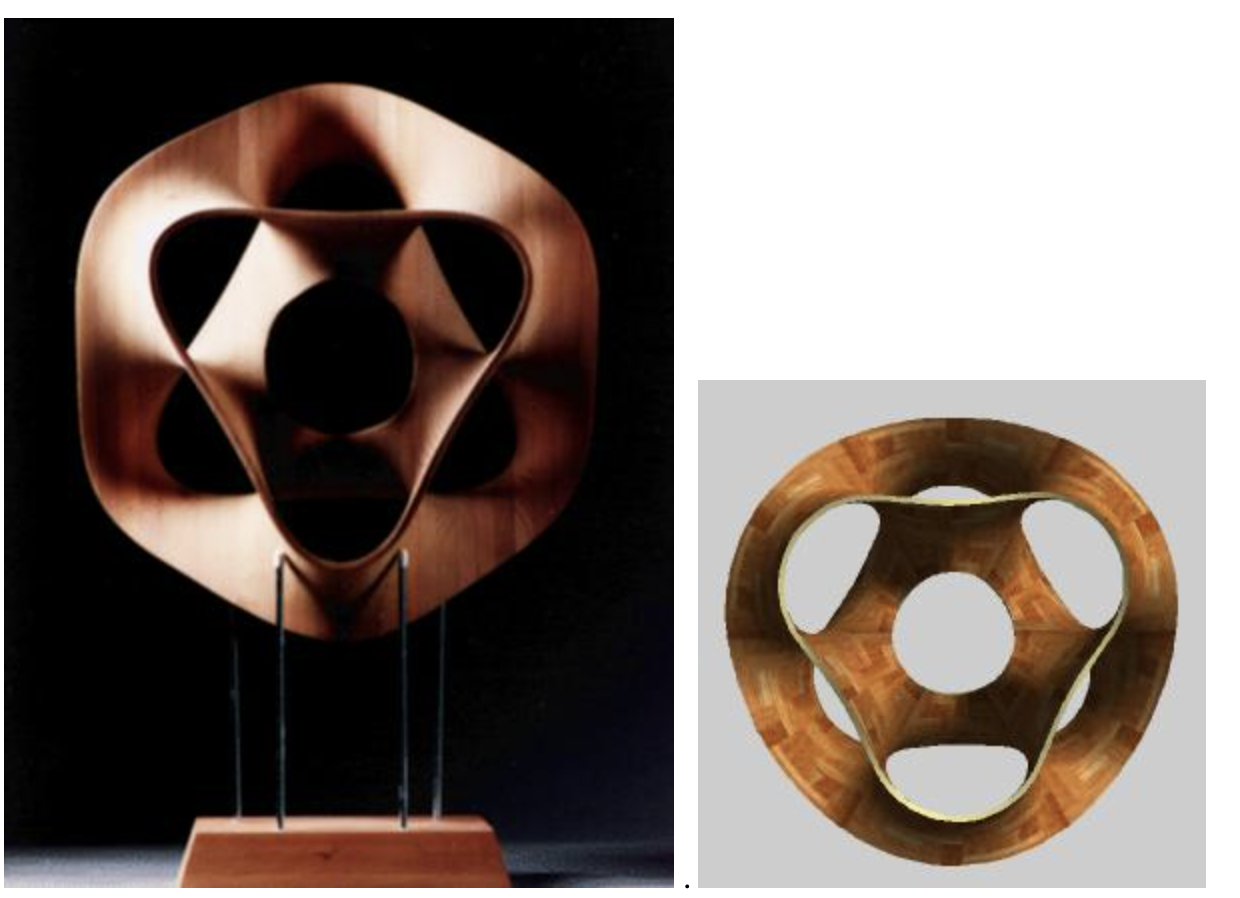
\includegraphics[scale=.4]{imagenes/6.png}
              
            \end{figure}
            \end{frame}
  %------------------------

\section{Propiedades importantes e interesantes}

  \begin{frame}
  \frametitle{Periodicidad}
  La periodicidad de las superficies de Scherk es evidente en las funciones de coseno y coseno presentes en sus formas paramétricas. Estas funciones son periódicas con periodos de $2\pi$ y $2\pi i$ respectivamente.
  \end{frame}
  
  \begin{frame}
  \frametitle{Introducción}
  La conjetura de Schoen-Yau fue una proposición en geometría hiperbólica, nombrada así por los matemáticos Richard Schoen y Shing-Tung Yau. Se inspiró en un teorema de Erhard Heinz en 1952, pero desde entonces ha sido refutada.
  \end{frame}
  
  \begin{frame}
  \frametitle{Configuración y Declaración de la Conjetura}
  Dejemos que $\mathbb{C}$ sea el plano complejo considerado como una variedad Riemanniana con su métrica Riemanniana usual (plana). Dejemos que $\mathbb{H}$ denote el plano hiperbólico, es decir, el disco unitario
  \[
  \mathbb{H}:=\{(x,y)\in \mathbb{R}^{2}|x^{2}+y^{2}<1\}
  \]
  dotado de la métrica hiperbólica
  \[
  ds^{2}=4\frac {dx^{2}+dy^{2}}{(1-(x^{2}+y^{2}))^{2}}.
  \]
  Heinz demostró que no puede existir ninguna difeomorfismo armónico $f:\mathbb{H}\to \mathbb{C}$. A la luz de este teorema, Schoen conjeturó que no existe ningún difeomorfismo armónico $g:\mathbb{C}\to \mathbb{H}$.
  \end{frame}
  

  

  \begin{frame}
  \frametitle{Refutación de la Conjetura}
  \begin{enumerate}
    \item La conjetura de Schoen-Yau fue refutada con el uso de superficies de Scherk. Harold Rosenberg y Pascal Collin en 2006 mostraron que existen difeomorfismos armónicos del plano complejo al plano hiperbólico utilizando superficies mínimas periódicas con simetría de traslación. 
    \item Esta prueba se basa en la convergencia de ciertas secuencias de superficies mínimas en el espacio euclidiano tridimensional, cuyos límites son difeomorfismos armónicos del plano complejo al plano hiperbólico.
  \end{enumerate}
  
  \end{frame}
  
  \begin{frame}
  \frametitle{Enneper-Weierstrass}
    Se pueden generar con la parametrización de Enneper-Weierstrass
  $$\left[\begin{array}{c}x(r, \phi) \\ y(r, \phi) \\ z(r, \phi)\end{array}\right]=\mathbb{R} \int\left[\begin{array}{c}f\left(1-g^2\right) \\ i f\left(1+g^2\right) \\ 2 f g\end{array}\right] d z$$

  donde $z= re^{i\phi}$ y $\mathcal{R}[z]$ es la parte real de $z$. 
  Para el caso particular de la segunda superficie de Scherk: $\frac{4}{1-z^4}$, $g(z)=iz$.
  \end{frame}

  
 \section{Superficies mínimas}

 \begin{frame}
  \frametitle{Lema importante}
  \begin{cajita}
    \begin{lema}
      Sea $S \subset \mathbb{R}^3$ superficie regular, con parámetros $(u, v)$ y $\mathbf{x}: U \subseteq \mathbb{R}^2 \rightarrow S$ su parametrización. Entonces,
      \begin{itemize}
        \item $\mathbf{x}$ es isotérmica $\Leftrightarrow F_1^2+F_2^2+F_3^2=0$.
        \item Si $\mathbf{x}$ es isotérmica, entonces $S$ es mínima $\Leftrightarrow F_1, F_2, F_3$ son holomorfas.
      \end{itemize}

    \end{lema}
  \end{cajita}

  \end{frame}
\begin{frame}
  \frametitle{Scherk 1}

  Dada por
$$
\mathbf{x}(t,\theta)=\left(\arg \frac{\zeta+i}{\zeta-i}, \arg \frac{\zeta+1}{\zeta-1}, \log \left|\frac{\zeta^2+1}{\zeta^2-1}\right|\right), \quad \zeta \neq \pm 1, \zeta \neq \pm i,
$$
donde $\zeta=u+i v$, y $\arg \zeta$ es el ángulo que el eje real hace con $\zeta$.

\end{frame}

\begin{frame}
  \frametitle{Scherk 1}

Calculamos que
$$
\begin{aligned}
\arg \frac{\zeta+i}{\zeta-i} & =\tan ^{-1} \frac{2 u}{u^2+v^2-1} \\
\arg \frac{\zeta+1}{\zeta-1} & =\tan ^{-1} \frac{-2 v}{u^2+v^2-1} \\
\log \left|\frac{\zeta^2+1}{\zeta^2-1}\right| & =\frac{1}{2} \log \frac{\left(u^2-v^2+1\right)^2+4 u^2 v^2}{\left(u^2-v^2-1\right)^2+4 u^2 v^2}
\end{aligned}
$$
por lo tanto,
$$
\varphi_1=\frac{\partial x}{\partial u}-i \frac{\partial x}{\partial v}=-\frac{2}{1+\zeta^2}, \quad \varphi_2=-\frac{2 i}{1-\zeta^2}, \quad \varphi_3=\frac{4 \zeta}{1-\zeta^4} .
$$
Dado que $\varphi_1^2+\varphi_2^2+\varphi_3^2 \equiv 0$ y $\varphi_1, \varphi_2$, y $\varphi_3$ son analíticos, $\mathbf{x}$ es una parametrización isotérmica de una superficie mínima.

\end{frame}
\begin{frame}
  \frametitle{Scherk 1}

  A partir de las expresiones de $x, y$, y $z$ que
$$
z=\log \frac{\cos y}{\cos x}
$$
Esta representación muestra que la superficie de Scherk se define en el patrón de ajedrez (excepto en los vértices de los cuadrados, donde la superficie es en realidad una línea vertical).

\end{frame}


\begin{frame}
  \frametitle{Scherk 1}
\begin{figure}
  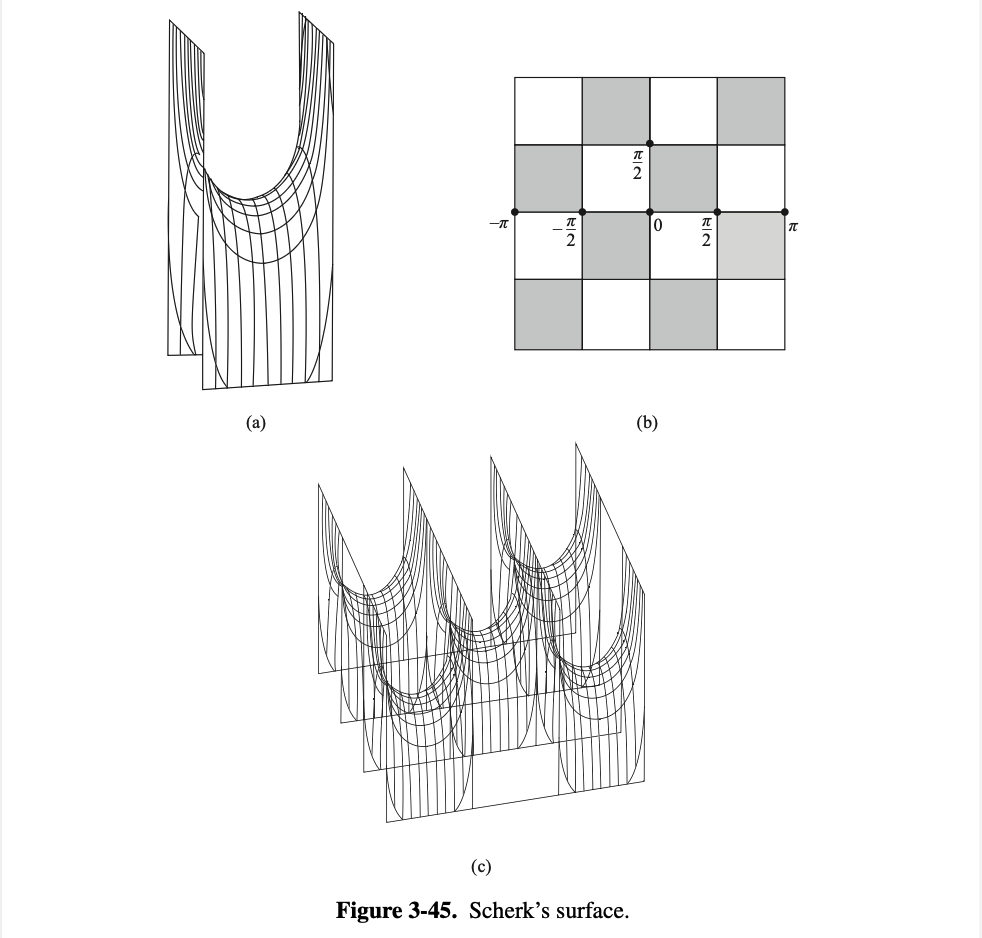
\includegraphics[scale=0.25]{imagenes/7.png}
\end{figure}

\end{frame}


\begin{frame}
  \frametitle{Laplaciano}
  \begin{cajita}
    \begin{definicion}
      El Laplaciano \(\Delta f\) de una función diferenciable \(f: U \subset R^2 \rightarrow R\) se define por \(\Delta f=\left(\partial^2 f / \partial u^2\right)+\left(\partial^2 f / \partial v^2\right),(u, v) \in U\). Decimos que \(f\) es armónica en \(U\) si \(\Delta f=0\).
    \end{definicion}
  \end{cajita}

  \end{frame}

  \begin{frame}
    \frametitle{Superficie mínima}

    \begin{cajita}
      \begin{corolario}
        Sea \(\mathbf{x}(\mathrm{u}, \mathrm{v})=(\mathrm{x}(\mathrm{u}, \mathrm{v}), \mathrm{y}(\mathrm{u}, \mathrm{v}), \mathrm{z}(\mathrm{u}, \mathrm{v}))\) una superficie parametrizada y supongamos que \(\mathbf{x}\) es isotérmica. Entonces \(\mathbf{x}\) es mínima si y solo si sus funciones de coordenadas \(\mathrm{x}, \mathrm{y}, \mathrm{z}\) son armónicas.
      \end{corolario}
    \end{cajita}
    \end{frame}

    
  
  \begin{frame}
    \frametitle{Superficie mínima: Scherk 2}

      Dado dado por
  $$
  \begin{aligned}
    \mathbf{x}(r,\theta)=\left( \ln \left( \frac{1+r^2+2r \cos \theta}{1+r^2-2r \cos \theta} \right), \frac{1+r^2-2r \sin\theta}{1+r^2+2r \sin \theta} , 2 \tan^{-1}\left( \frac{2 r^2 \sin 2\theta}{r^4} \right)\right)
  \end{aligned}
  $$

  \end{frame}
  \begin{frame}
    
    \begin{align*}
      x_r &= \left( \frac{-4 (-1 + r^2) \cos(\theta)}{1 + r^4 - 2 r^2 \cos(2 \theta)}, \frac{4 (-1 + r^2) \sin(\theta)}{1 + r^4 + 2 r^2 \cos(2 \theta)},\right. \\
      &\quad \left.\frac{-8 r \sin(2 \theta)}{r^4 + 4 \sin(2 \theta)^2} \right)\\
      x_\theta &= \left( \frac{-4 r (1 + r^2) \sin(\theta)}{1 + r^4 - 2 r^2 \cos(2 \theta)}, \frac{-4 r (1 + r^2) \cos(\theta)}{1 + r^4 + 2 r^2 \cos(2 \theta)},\right.\\
      &\quad\left.\frac{8 r^2 \cos(2 \theta)}{r^4 + 4 \sin(2 \theta)^2} \right)\\
      x_{rr} &= \left( \frac{8 r \cos(\theta) (-1 - 2 r^2 + r^4 + 2 \cos(2 \theta))}{(1 + r^4 - 2 r^2 \cos(2 \theta))^2},\right.\\
      &\quad \left.\frac{8 r (-(r^2 (-2 + r^2) \sin(\theta)) + \sin(3 \theta))}{(1 + r^4 + 2 r^2 \cos(2 \theta))^2}, \frac{8 (-2 + 3 r^4 + 2 \cos(4 \theta)) \sin(2 \theta)}{(r^4 + 4 \sin(2 \theta)^2)^2} \right)
    \end{align*}
  \end{frame}


  \begin{frame}
    \begin{align*}
      x_{\theta\theta} &= \left( \frac{-4 r (1 + r^2) \cos(\theta) (1 - 4 r^2 + r^4 + 2 r^2 \cos(2 \theta))}{(1 + r^4 - 2 r^2 \cos(2 \theta))^2},\right.\\
      &\quad\frac{4 r (1 + r^2) ((1 - 3 r^2 + r^4) \sin(\theta) - r^2 \sin(3 \theta))}{(1 + r^4 + 2 r^2 \cos(2 \theta))^2},\\
      &\left. \frac{-16 r^2 (6 + r^4 + 2 \cos(4 \theta)) \sin(2 \theta)}{(r^4 + 4 \sin(2 \theta)^2)^2} \right)\\
      x_{r\theta} &= \left( \frac{4 (-1 + r^2) (1 + 4 r^2 + r^4 + 2 r^2 \cos(2 \theta)) \sin(\theta)}{(1 + r^4 - 2 r^2 \cos(2 \theta))^2},\right. \\
      & \frac{4 (-1 + r^2) \cos(\theta) (1 + 4 r^2 + r^4 - 2 r^2 \cos(2 \theta))}{(1 + r^4 + 2 r^2 \cos(2 \theta))^2}, \\
      &\left.\quad \frac{-16 r \cos(2 \theta) (-2 + r^4 + 2 \cos(4 \theta))}{(r^4 + 4 \sin(2 \theta)^2)^2} \right)
    \end{align*}
    
      \end{frame}


      \begin{frame}
        \begin{align*}
          x_{\theta r} &= \left( \frac{4 (-1 + r^2) (1 + 4 r^2 + r^4 + 2 r^2 \cos(2 \theta)) \sin(\theta)}{(1 + r^4 - 2 r^2 \cos(2 \theta))^2},\right.\\
          & \frac{4 (-1 + r^2) \cos(\theta) (1 + 4 r^2 + r^4 - 2 r^2 \cos(2 \theta))}{(1 + r^4 + 2 r^2 \cos(2 \theta))^2},\\
          &\left. \frac{-16 r \cos(2 \theta) (-2 + r^4 + 2 \cos(4 \theta))}{(r^4 + 4 \sin(2 \theta)^2)^2} \right)
        \end{align*}
        
          \end{frame}

  \begin{frame}
    \frametitle{Superficie mínima: Scherk 2}

  Primera forma    $$
\begin{aligned}
& E=\frac{16\left(1+r^2\right)^2}{1+r^8-2 r^4 \cos (4 \phi)} \\
& F=0 \\
& G=\frac{16 r^2\left(1+r^2\right)^2}{1+r^8-2 r^4 \cos (4 \phi)}
\end{aligned}
$$
Segunda forma 
$$
\begin{gathered}
e=\frac{8\left(1+r^4\right) \sin (2 \phi)}{1+r^8-2 r^4 \cos (4 \phi)} \\
f=\frac{8\left(1-r^4\right) \cos (2 \phi)}{1+r^8-2 r^4 \cos (4 \phi)} \\
g=\frac{8 r^2\left(1+r^4\right) \sin (2 \phi)}{1+r^8-2 r^4 \cos (4 \phi)} .
\end{gathered}
$$


  \end{frame}

  \begin{frame}
    \frametitle{Superficie mínima: Scherk 2}


   Curvatura media y gaussiana
    $$
    \begin{aligned}
    & K=-\frac{1+r^8-2 r^4 \cos (4 \phi)}{4\left(1+r^2\right)^4} \\
    & H=0 .
    \end{aligned}
    $$

  \end{frame}
  
  

  %-------------------------------
  
  \begin{frame}{Curvatura Media Cero}
    \begin{cajita}
      \begin{definicion}
        Sea $S \subseteq \mathbb{R}^3$ superficie regular, $\mathbf{p} \in S$. Sean $\kappa_1 y \kappa_2$ las curvaturas principales de $S$ en $\mathbf{p}$. Definimos la curvatura media de $S$ en $\mathbf{p}$ como
  $$
  H=\frac{1}{2}\left(\kappa_1+\kappa_2\right)=-\frac{1}{2} \operatorname{tr} D N(\mathbf{p}) .
  $$
  Definimos la curvatura de Gauss de $S$ en $\mathbf{p}$ como
  $$
  K=\kappa_1 \kappa_2=\operatorname{det} D N(\mathbf{p})
  $$
      \end{definicion}
    \end{cajita}
    
    
 \end{frame}

 \begin{frame}{Curvatura Media Cero}

  \begin{itemize}
    \item Para una superficie mínima, la curvatura media es cero en cada punto, es decir, $H = \frac{k_1 + k_2}{2} = 0$.
    \item Por lo tanto, para la superficie Scherk 1 y Scherk 2, las curvaturas principales en cada punto deben ser opuestas entre sí, es decir, $k_1 = -k_2$.
\end{itemize}
\end{frame}



 \begin{frame}{Referencias}
  \begin{itemize}
    \item Do Carmo, M. P. (2016). Differential geometry of curves and surfaces: Revised and updated second edition. Dover Publications.
    \item Gray, A. "Minimal Surfaces via the Weierstrass Representation." Ch. 32 in Modern Differential Geometry of Curves and Surfaces with Mathematica, 2nd ed. Boca Raton, FL: CRC Press, pp. 735-760, 1997
    \item Hazewinkel, Michiel, ed. (2001), "Scherk surface", Encyclopedia of Mathematics, Springer Science+Business Media B.V. /
  \end{itemize}
 \end{frame}




\end{document}
